%!TEX root = ./template-skripsi.tex

\subsection{Sprint 3 Report}
Berikut merupakan report dari sprint ke-3 yang dilakukan pada tanggal 8 juni - 14 juni 2022.

\begin{table}[H]
	\caption{\textit{Sprint-3 backlog}}
	\label{sprint3_backlog}
	\begin{tabular}{@{} |p{0.5cm}|p{5cm}|p{5cm}|p{2cm}| @{}}
		\hline
		\textbf{No} & \textbf{\textit{Story}} & \textbf{\textit{Task}} & \textbf{\textit{Status}} \\
		\hline
		1 & \multirow{3}{5cm}{Create, Read, Updte, dan Delete untuk Registrasi kolam} & Membarui desain database  & Completed\\
		\cline{1-1}\cline{3-4}
		2 & & Membarui API entry kolam & Completed\\
		\cline{1-1}\cline{3-4}
		3 & & Membarui API edit kolam & Completed\\
		\cline{1-1}\cline{3-4}
		4 & & Membarui API fetch list kolam & Completed\\
		\cline{1-1}\cline{3-4}
		5 & & Membuat API edit foto kolam & Completed\\
		\cline{1-1}\cline{3-4}
		6 & & Membuat API fetch foto kolam & Completed\\
		\cline{1-1}\cline{3-4}
		7 & & Membuat View detail kolam & Completed\\
		\cline{1-1}\cline{3-4}
		\hline
	\end{tabular}
\end{table}

\begin{enumerate}[1.]

\item Desain database
\begin{figure}[H]
	\centering
	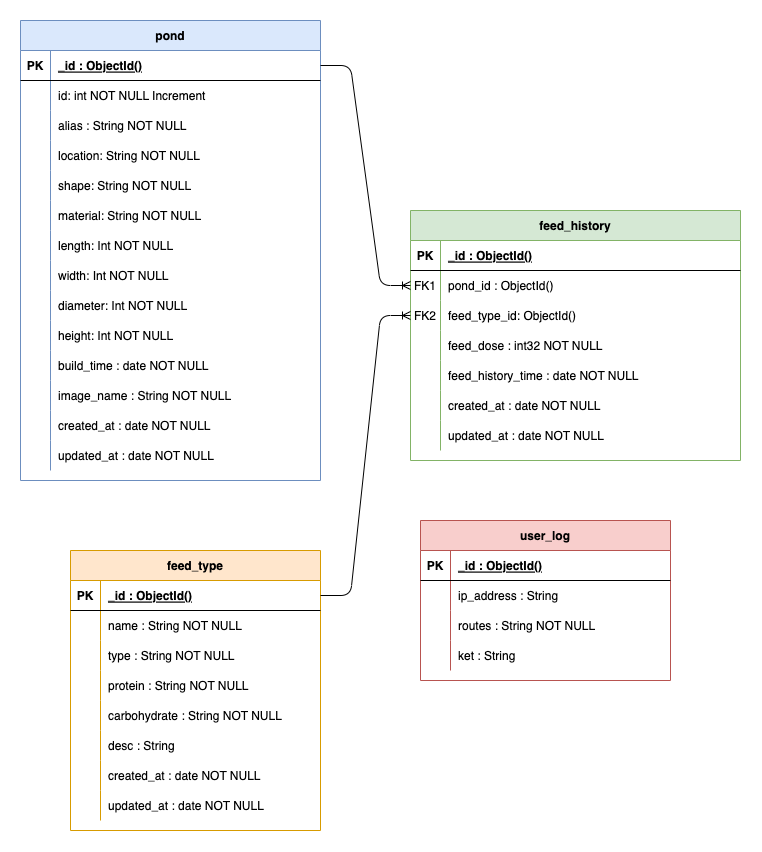
\includegraphics[height=0.7\textwidth]{gambar/Sprint03/diagram database/database}
	\caption{ERD Database Sprint-3}
	\label{fig:database_sprint3}
\end{figure}

Dengan berubahnya desain database diperlukan juga perubahan model pada source code, berikut perubahan pada source code model kolam.

\begin{lstlisting}
# fishapi/database/model.py

class Pond(db.Document):
    id_int = db.SequenceField(required=True)
    alias = db.StringField(required=True)
    location = db.StringField(required=True)
    shape = db.StringField(required=True)
    material = db.StringField(required=True)
    length = db.FloatField(required=True, default=0)
    width = db.FloatField(required=True, default=0)
    diameter = db.FloatField(required=True, default=0)
    height = db.FloatField(required=True, default=0)
    image_name = db.StringField(required=True, default='default.jpg')
    build_at = db.DateTimeField(default=datetime.datetime.now)
    created_at = db.DateTimeField(default=datetime.datetime.now)
    updated_at = db.DateTimeField(default=datetime.datetime.now)
\end{lstlisting}

\item Membarui API entry kolam

Perubahan terjadi pada controller API entry kolam, berikut merupakan perubahan source code controller API entry kolam.
\begin{lstlisting}
# fishapi/resources/controller/pond.py

def post(self):
        try:
            body = {
                "alias": request.form.get("alias", None),
                "location": request.form.get("location", None),
                "shape": request.form.get("shape", None),
                "material": request.form.get("material", None),
                "length": request.form.get("length", None),
                "width": request.form.get("width", None),
                "diameter": request.form.get("diameter", None),
                "height": request.form.get("height", None),
                "build_at": request.form.get("build_at", None),
            }
            pond = Pond(**body).save()
            id = pond.id
            response = {"message": "success add pond", "id": id}
            response = json.dumps(response, default=str)
            return Response(response, mimetype="application/json", status=200)
        except Exception as e:
            response = {"message": str(e)}
            response = json.dumps(response, default=str)
            return Response(response, mimetype="application/json", status=400)
\end{lstlisting}

Fungsi ini merupakan sebuah endpoint HTTP POST yang digunakan untuk menambahkan data kolam ke dalam database.

Pada bagian awal fungsi, request.form.get digunakan untuk membaca nilai dari setiap parameter dari request yang dikirim melalui form-data. Nilai-nilai ini kemudian digabungkan menjadi satu objek body.

Kemudian, objek Pond yang baru dibuat dengan parameter yang diambil dari objek body tersebut. Setelah itu, fungsi "save()" digunakan untuk menyimpan objek Pond ke dalam database.

Jika operasi penyimpanan berhasil dilakukan, fungsi akan memberikan respons dengan status kode 200 dan pesan "success add pond" beserta ID dari kolam yang baru saja ditambahkan. Jika terjadi kesalahan dalam proses ini, fungsi akan memberikan respons dengan status kode 400 dan pesan kesalahan dalam format JSON.

Fungsi json.dumps() digunakan untuk mengkonversi objek response ke dalam format JSON dan menentukan parameter default=str agar objek dapat di-serialize dalam format JSON. Terakhir, fungsi mengembalikan respons dengan header "application/json".

Berikut merupakan form untuk entry kolam.

% Please add the following required packages to your document preamble:
% \usepackage[table,xcdraw]{xcolor}
% If you use beamer only pass "xcolor=table" option, i.e. \documentclass[xcolor=table]{beamer}
\begin{table}[]
\begin{tabular}{|l|l|l|}
\hline
\multicolumn{1}{|c|}{\cellcolor[HTML]{F9F9F9}\textbf{Form}} & \multicolumn{1}{c|}{\cellcolor[HTML]{F9F9F9}\textbf{Jenis}}                                                               & \textbf{Deskripsi}     \\ \hline
{\color[HTML]{212121} alias}                                & {\color[HTML]{212121} REQUIRED STRING}                                                                                    & alias/nama untuk kolam \\ \hline
{\color[HTML]{212121} location}                             & {\color[HTML]{212121} REQUIRED STRING}                                                                                    & lokasi kolam           \\ \hline
{\color[HTML]{212121} shape}                                & {\color[HTML]{212121} \begin{tabular}[c]{@{}l@{}}REQUIRED STRING\\ VALUE : {[}'persegi', 'bundar'{]}\end{tabular}}        & bentuk kolam           \\ \hline
{\color[HTML]{212121} material}                             & {\color[HTML]{212121} \begin{tabular}[c]{@{}l@{}}REQUIRED STRING\\ VALUE : {[}'tanah', 'terpal', 'beton'{]}\end{tabular}} & bahan bangun kolam     \\ \hline
{\color[HTML]{212121} length}                               & {\color[HTML]{212121} REQUIRED DOUBLE FOR SHAPE ('peresgi')}                                                              & panjang kolam          \\ \hline
{\color[HTML]{212121} width}                                & {\color[HTML]{212121} REQUIRED DOUBLE FOR SHAPE ('peresgi')}                                                              & lebar kolam            \\ \hline
{\color[HTML]{212121} diameter}                             & {\color[HTML]{212121} REQUIRED DOUBLE FOR SHAPE ('bundar')}                                                               & diameter kolam         \\ \hline
{\color[HTML]{212121} height}                               & {\color[HTML]{212121} REQUIRED DOUBLE}                                                                                    & tinggi kolam           \\ \hline
{\color[HTML]{212121} build\_at}                            & {\color[HTML]{212121} \begin{tabular}[c]{@{}l@{}}OPTIONAL STRING\\ DATETIME \{YYYY-mm-dd THH:MM:ss\}\end{tabular}}        & tanggal kolam dibuat   \\ \hline
\end{tabular}
\end{table}

Tabel tersebut menjelaskan parameter-parameter yang dibutuhkan untuk membuat suatu kolam dalam suatu program atau sistem. Setiap baris di tabel tersebut menjelaskan satu parameter yang diperlukan untuk membuat kolam, yang terdiri dari tiga kolom:

\begin{enumerate}[a.]
\item Form: kolom ini menjelaskan nama parameter yang dibutuhkan untuk membuat kolam
\item Jenis: kolom ini menjelaskan jenis data yang diperlukan untuk nilai parameter tersebut, termasuk apakah data tersebut wajib atau opsional, dan jika wajib, tipe data apa yang harus digunakan.
\item Deskripsi: kolom ini memberikan deskripsi singkat tentang arti parameter tersebut.
\end{enumerate}

Dalam tabel tersebut, terdapat sembilan parameter yang dibutuhkan untuk membuat kolam, yaitu "alias", "location", "shape", "material", "length", "width", "diameter", "height", dan "build\_at". Beberapa parameter adalah wajib, seperti "alias", "location", "shape", "material", dan "height", sedangkan beberapa parameter lainnya adalah opsional, seperti "build\_at". Terdapat juga beberapa parameter yang memerlukan jenis data khusus, seperti "shape" yang harus bernilai "persegi" atau "bundar", dan "build\_at" yang harus merupakan datetime dalam format tertentu.

Berikut merupakan hasil test request dari API entry kolam.

cURL:

\begin{lstlisting}
curl --location 'http://jft.web.id/fishapi/api/ponds' \
--form 'alias="epsilon"' \
--form 'location="blok 3"' \
--form 'shape="persegi"' \
--form 'material="tanah"' \
--form 'length="5"' \
--form 'width="3"' \
--form 'height="0.7"'
\end{lstlisting}

response json:

\begin{lstlisting}
{
  "message": "success add pond",
  "id": "62aa118fa95cbcb494c5a4a6"
}\end{lstlisting}

\item Membarui API edit kolam

Perubahan terjadi pada controller API edit kolam, berikut merupakan perubahan source code controller API edit kolam.

\begin{lstlisting}
# fishapi/resources/controller/pond.py

def put(self, id):
        try:
            body = request.form.to_dict(flat=True)
            Pond.objects.get(id=id).update(**body)
            response = {"message": "success change data pond", "id": id}
            response = json.dumps(response, default=str)
            return Response(response, mimetype="application/json", status=200)
        except Exception as e:
            response = {"message": str(e)}
            response = json.dumps(response, default=str)
            return Response(response, mimetype="application/json", status=400)
        return
\end{lstlisting}

Fungsi ini merupakan sebuah endpoint HTTP PUT yang digunakan untuk mengubah data kolam yang sudah ada di dalam database.

Saat endpoint ini dipanggil, fungsi akan membaca input yang diberikan melalui form-data dan membuat objek body dengan nilai-nilai parameter tersebut.

Kemudian, fungsi "update()" pada objek Pond yang memiliki ID yang sesuai akan dipanggil dengan parameter nilai-nilai dari objek body tersebut. Fungsi ini akan mengubah nilai dari setiap parameter yang terkait dengan ID kolam tersebut di dalam database.

Jika operasi pengubahan berhasil dilakukan, fungsi akan memberikan respons dengan status kode 200 dan pesan "success change data pond" beserta ID dari kolam yang diubah. Jika terjadi kesalahan dalam proses ini, fungsi akan memberikan respons dengan status kode 400 dan pesan kesalahan dalam format JSON.

Fungsi json.dumps() digunakan untuk mengkonversi objek response ke dalam format JSON dan menentukan parameter default=str agar objek dapat di-serialize dalam format JSON. Terakhir, fungsi mengembalikan respons dengan header "application/json".

Berikut merupakan hasil test request yang dari API edit kolam.

cURL:

\begin{lstlisting}
curl --location -g --request PUT 'http://jft.web.id/fishapi/api/ponds/{pond_id}' \
--form 'material="terpal"'
\end{lstlisting}

response json:

\begin{lstlisting}
{
  "message": "success change data pond",
  "id": "625d7033a9a73e090c65cda2"
}
\end{lstlisting}

\item Membarui API fetch list kolam

Perubahan terjadi pada controller API fetch list kolam, berikut merupakan perubahan source code controller API fetch list kolam.

\begin{lstlisting}
# fishapi/resources/controller/pond.py

def get(self):
        try:
            url = url_for('pondimageapidummy', _external=True)
            pipeline = [
                {"$addFields": {
                    "area": {"$cond": {
                        "if": {"$eq": ["$shape", "persegi"]},
                        "then": {"$multiply": ["$length", "$width"]},
                        "else": {"$divide": [
                            {"$multiply": [22, "$diameter", "$diameter"]},
                            28
                        ]},
                    }},
                    "image_link":{"$concat": [url, "/", {"$toString": "$_id"}]}
                }},
                {"$addFields": {
                    "volume": {"$multiply": ["$area", "$height"]}
                }},
                {"$project": {
                    "pond_id": 0,
                    "feed_type_id": 0,
                    "created_at": 0,
                    "updated_at": 0,
                }}
            ]
            ponds = Pond.objects.aggregate(pipeline)
            list_ponds = list(ponds)
            response = json.dumps(list_ponds, default=str)
            return Response(response, mimetype="application/json", status=200)
        except Exception as e:
            response = {"message": str(e)}
            response = json.dumps(response, default=str)
            return Response(response, mimetype="application/json", status=400)\end{lstlisting}
            
Fungsi ini merupakan sebuah endpoint HTTP GET yang digunakan untuk mengambil data kolam yang sudah ada di dalam database.

Saat endpoint ini dipanggil, fungsi akan melakukan query terhadap database untuk mengambil data kolam yang sudah ada. Query ini dilakukan dengan menggunakan objek pipeline yang akan menambahkan field "area" dan "image\_link" pada hasil query.

Field "area" akan diisi dengan nilai luas kolam yang dihitung berdasarkan shape, length, width, dan diameter kolam. Field "image\_link" akan diisi dengan URL gambar kolam yang diambil dari endpoint "pondimageapidummy".

Setelah itu, field "volume" akan ditambahkan ke hasil query dengan menghitung nilai volume kolam berdasarkan field "area" dan "height".

Terakhir, hasil query akan diproyeksikan ke dalam objek yang hanya mengandung field-field tertentu saja seperti "alias", "location", "shape", "material", "length", "width", "diameter", "height", "area", "volume", dan "image\_link".

Jika query berhasil dilakukan, fungsi akan memberikan respons dengan status kode 200 dan daftar kolam dalam format JSON. Jika terjadi kesalahan dalam proses ini, fungsi akan memberikan respons dengan status kode 400 dan pesan kesalahan dalam format JSON.

Berikut merupakan hasil test request yang dari API fetch list kolam.

cURL:

\begin{lstlisting}
curl --location 'http://jft.web.id/fishapi/api/ponds'
\end{lstlisting}

response json:

\begin{lstlisting}
[
  {
    "_id": "625d7026a9a73e090c65cda1",
    "id_int": 2,
    "alias": "alpha",
    "location": "blok 1",
    "shape": "bundar",
    "material": "beton",
    "length": 0,
    "width": 0,
    "diameter": 1.4,
    "height": 1,
    "build_at": "2022-04-18 21:05:26.183000",
    "image_name": "kolam_1655141767.jpeg",
    "area": 1.5399999999999998,
    "image_link": "http://127.0.0.1:5000/api/ponds/image/625d7026a9a73e090c65cda1",
    "volume": 1.5399999999999998
  },
  {
    "_id": "625d7033a9a73e090c65cda2",
    "id_int": 3,
    "alias": "beta",
    "location": "blok 1",
    "shape": "persegi",
    "material": "terpal",
    "length": 8,
    "width": 4,
    "diameter": 0,
    "height": 1,
    "build_at": "2022-04-18 21:05:39.608000",
    "image_name": "default.jpg",
    "area": 32,
    "image_link": "http://127.0.0.1:5000/api/ponds/image/625d7033a9a73e090c65cda2",
    "volume": 32
  },
  {......
]
\end{lstlisting}

\item Menambahkan API edit foto kolam

Penambahan API untuk fungsi edit foto kolam, berikut merupakan penambahan source code controller API edit foto kolam.

\begin{lstlisting}
# fishapi/resources/controller/pond.py

def put(self, id):
        try:
            file = request.files['image']
            if not file:
                response = {"message": "no file selected"}
                response = json.dumps(response, default=str)
                return Response(response, mimetype="application/json", status=400)
            if not allowed_file(file.filename):
                response = {"message": "file type not allowed"}
                response = json.dumps(response, default=str)
                return Response(response, mimetype="application/json", status=400)
            filename = secure_filename(file.filename)
            filename = pad_timestamp(filename)
            path = os.path.join(current_app.instance_path,
                                current_app.config['UPLOAD_DIR'])
            try:
                os.makedirs(path)
            except OSError:
                pass
            filepath = os.path.join(path, filename)
            file.save(filepath)
            # database
            objects = Pond.objects.get(id=id)
            pond = objects.to_mongo()
            old_image_name = pond["image_name"]
            new_image_name = filename
            if old_image_name != "default.jpg":
                os.remove(os.path.join(path, old_image_name))
            data = {
                "image_name": new_image_name
            }
            objects.update(**data)
            id = objects.id
            response = {"message": "success change image", "id": id}
            response = json.dumps(response, default=str)
            return Response(response, mimetype="application/json", status=200)
        except Exception as e:
            response = {"message": str(e)}
            response = json.dumps(response, default=str)
            return Response(response, mimetype="application/json", status=400)
\end{lstlisting}

Kode tersebut merupakan implementasi dari method PUT pada API untuk mengganti gambar kolam ikan berdasarkan ID kolam. Pertama, API akan menerima request PUT yang berisi file gambar yang ingin diganti dan ID kolam yang ingin diubah gambarnya. Jika tidak ada file gambar yang dipilih, maka akan mengembalikan response "no file selected" dengan status code 400. Jika file yang dipilih tidak diperbolehkan, maka akan mengembalikan response "file type not allowed" dengan status code 400.

Selanjutnya, filename dari file gambar tersebut akan diproses dengan fungsi secure\_filename dan pad\_timestamp untuk memastikan nama file yang aman dan unik. Path untuk menyimpan file gambar akan dibuat, dan file akan disimpan di path tersebut.

Kemudian, API akan mengambil data kolam ikan berdasarkan ID yang diberikan dari database. Gambar lama dari kolam ikan tersebut akan dihapus jika bukan "default.jpg" dan digantikan dengan gambar baru yang telah dipilih.

Terakhir, API akan mengembalikan response "success change image" beserta ID kolam ikan yang diubah gambarnya dengan status code 200. Jika terjadi error pada proses ini, maka akan mengembalikan response dengan pesan error dan status code 400.

Berikut merupakan hasil test request yang dari API edit foto kolam. Simulasi dibuat dengan mengisikan form 'image' dengan path image yang ada di direktori local user.

cURL:

\begin{lstlisting}
curl --location -g --request PUT 'http://jft.web.id/fishapi/api/ponds/image/{pond_id}' \
--form 'image=@"/Users/andrirahmanto/Downloads/kolam.jpeg"'
\end{lstlisting}

response json:

\begin{lstlisting}
{
  "message": "success change image",
  "id": "62a62163e445ffb9c5f746f3"
}
\end{lstlisting}

\item Membuat View detail kolam

\begin{figure}[H]
	\centering
	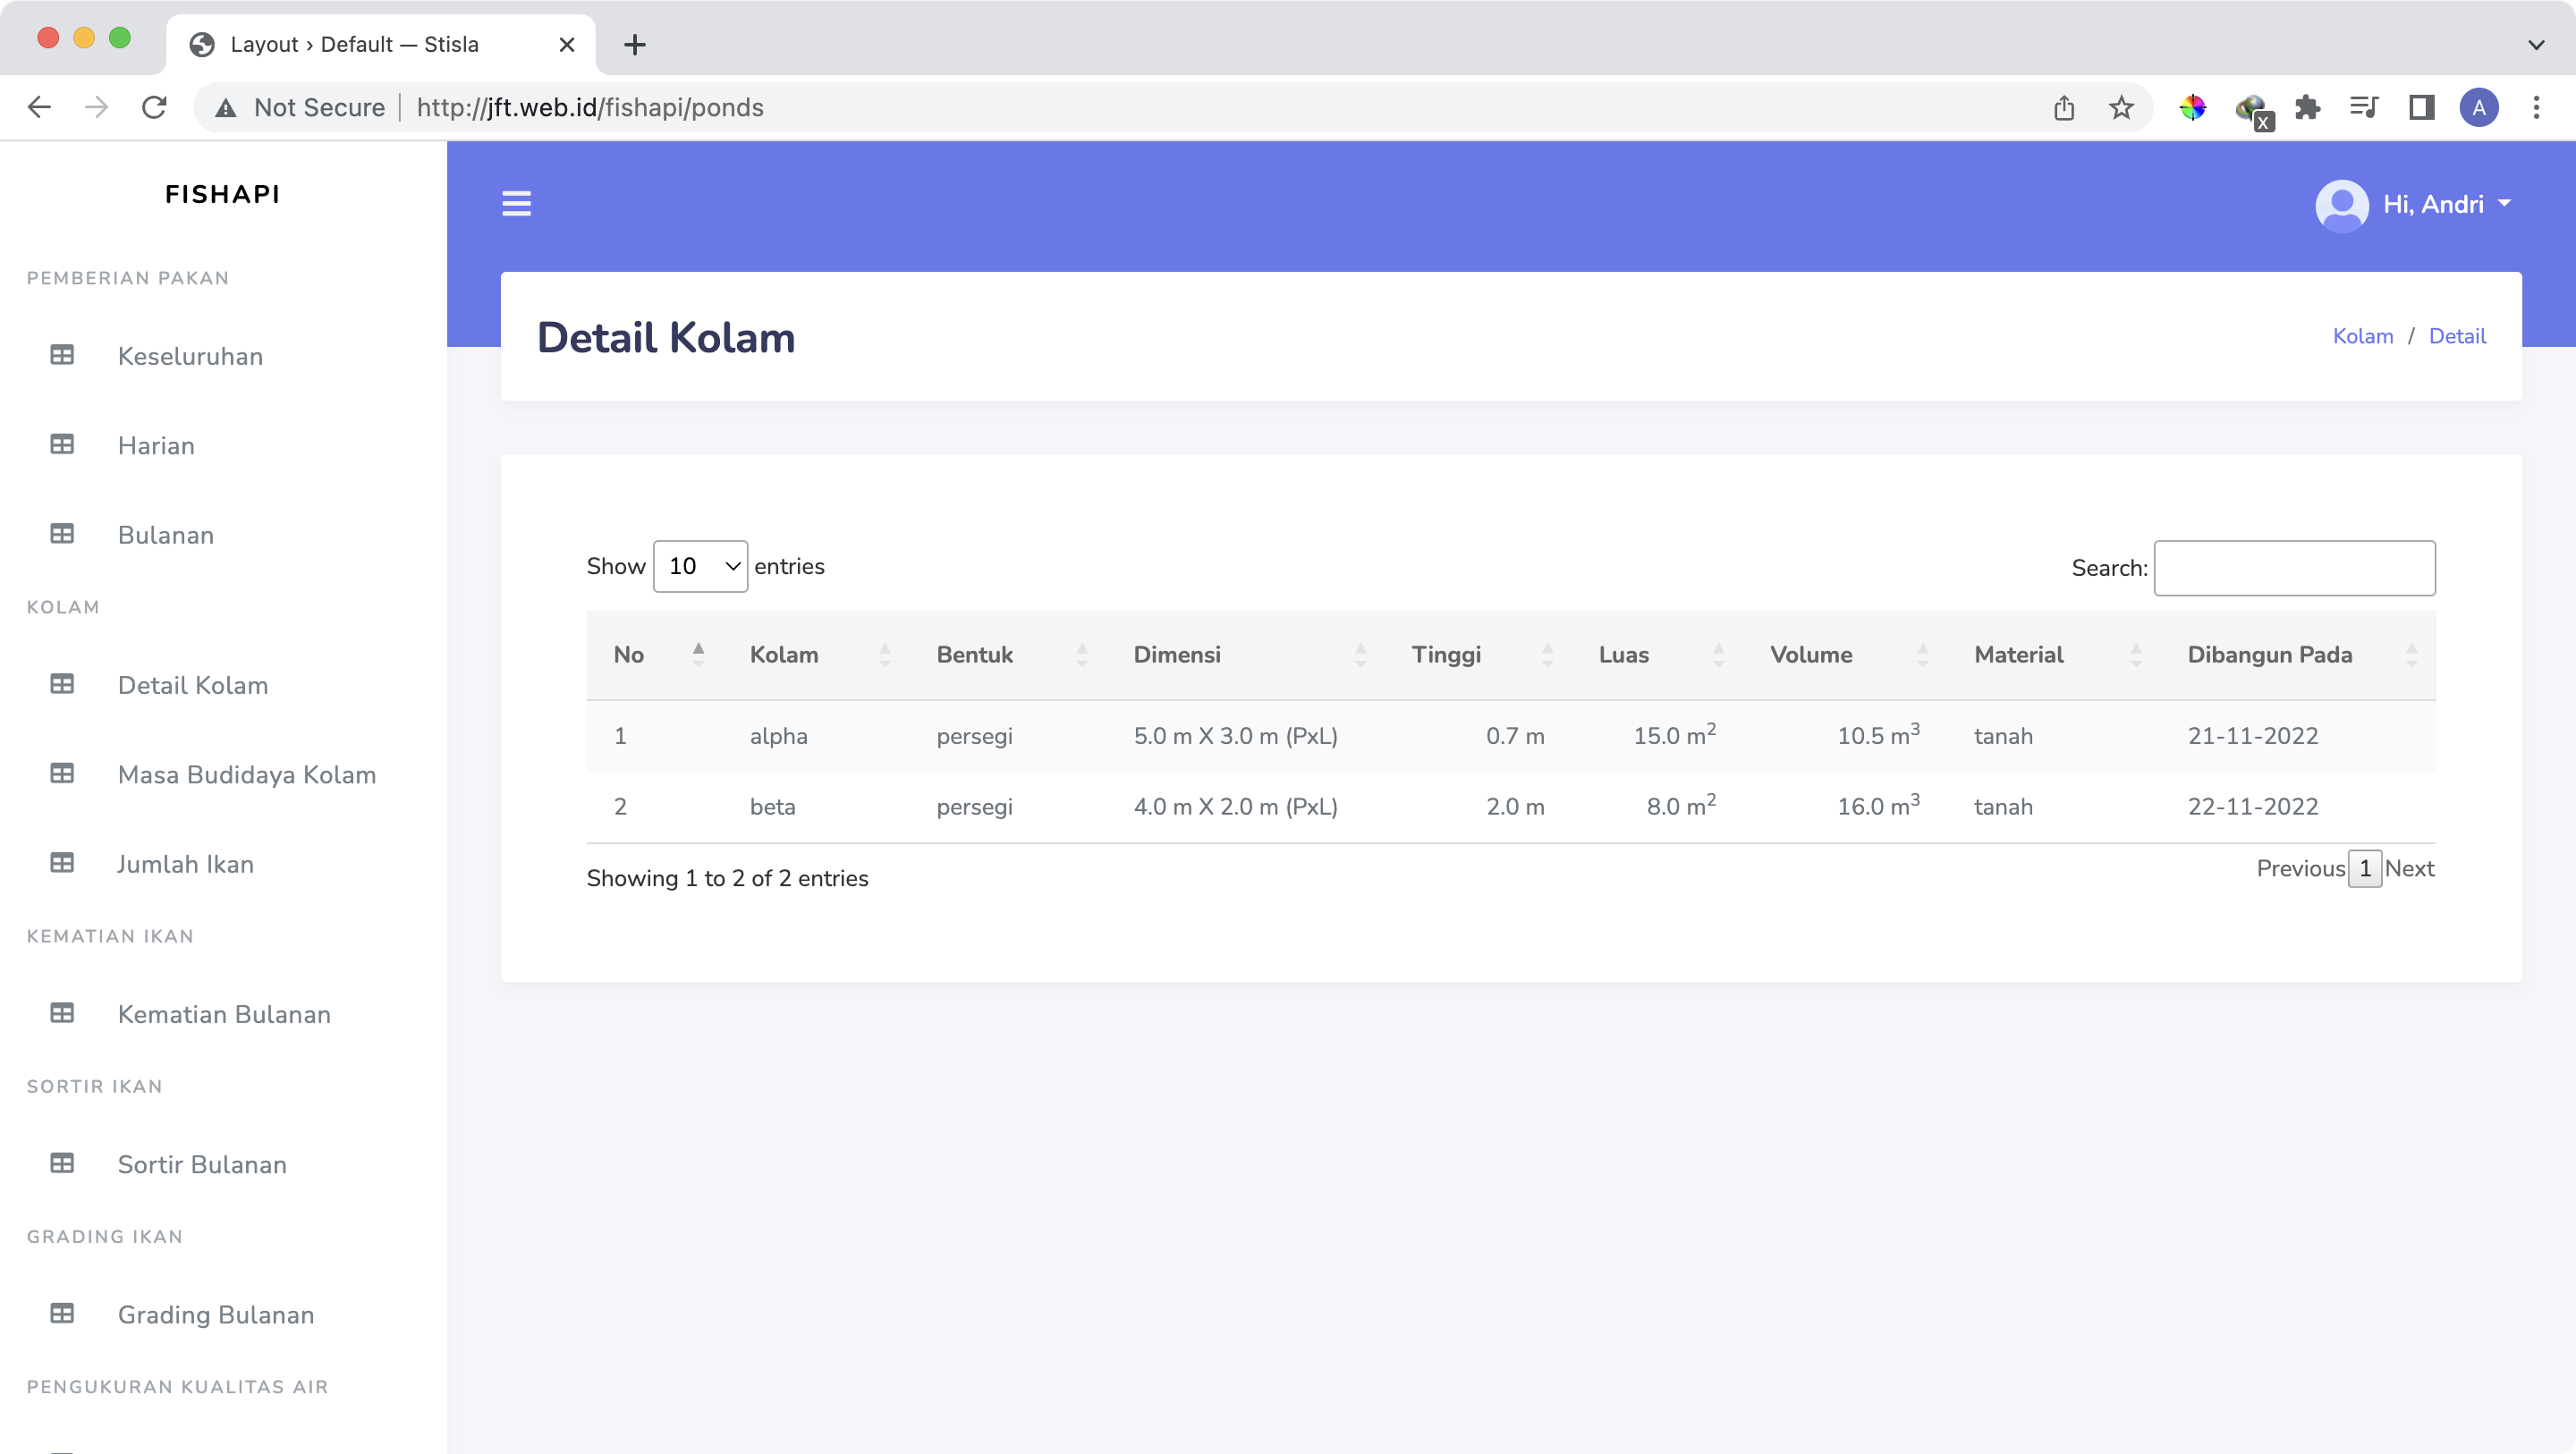
\includegraphics[width=1\textwidth]{gambar/Sprint03/view/view_detail_kolam}
	\caption{View detail kolam}
	\label{fig:view_detail_kolam}
\end{figure}
	
\end{enumerate}